% !TeX root = main.tex
\chapter{Results}
 Since we want to study the attributes and the occurrence of premature stop codons in the 1,135 population of \textit{A. thaliana} we try to characterize how natural selection is shaping population structures through loss-of-function variants. To answer this research question we followed an statistical workflow. We will start the project by looking first at the distribution of premature stop codons in the 1, 135 accessions of \textit{A.thaliana} dataset and continue by generating two high confidential datasets for our further analysis. Here we will follow two separate approaches, one is based on the gene expression differences between wildtype and knock-out mutants the other one by selecting stop codons based on the calculation of the remaining length. Afterwards we want to look at the interactions between premature stop codons and finish our analysis by looking at a control group of mutations, which will be the synonymous mutations. 
\section{Distribution of premature stop codons in \textit{A. thaliana}}

\begin{figure}[tb]
    \centering
    \begin{minipage}[h]{0.9\textwidth}
      \centering
      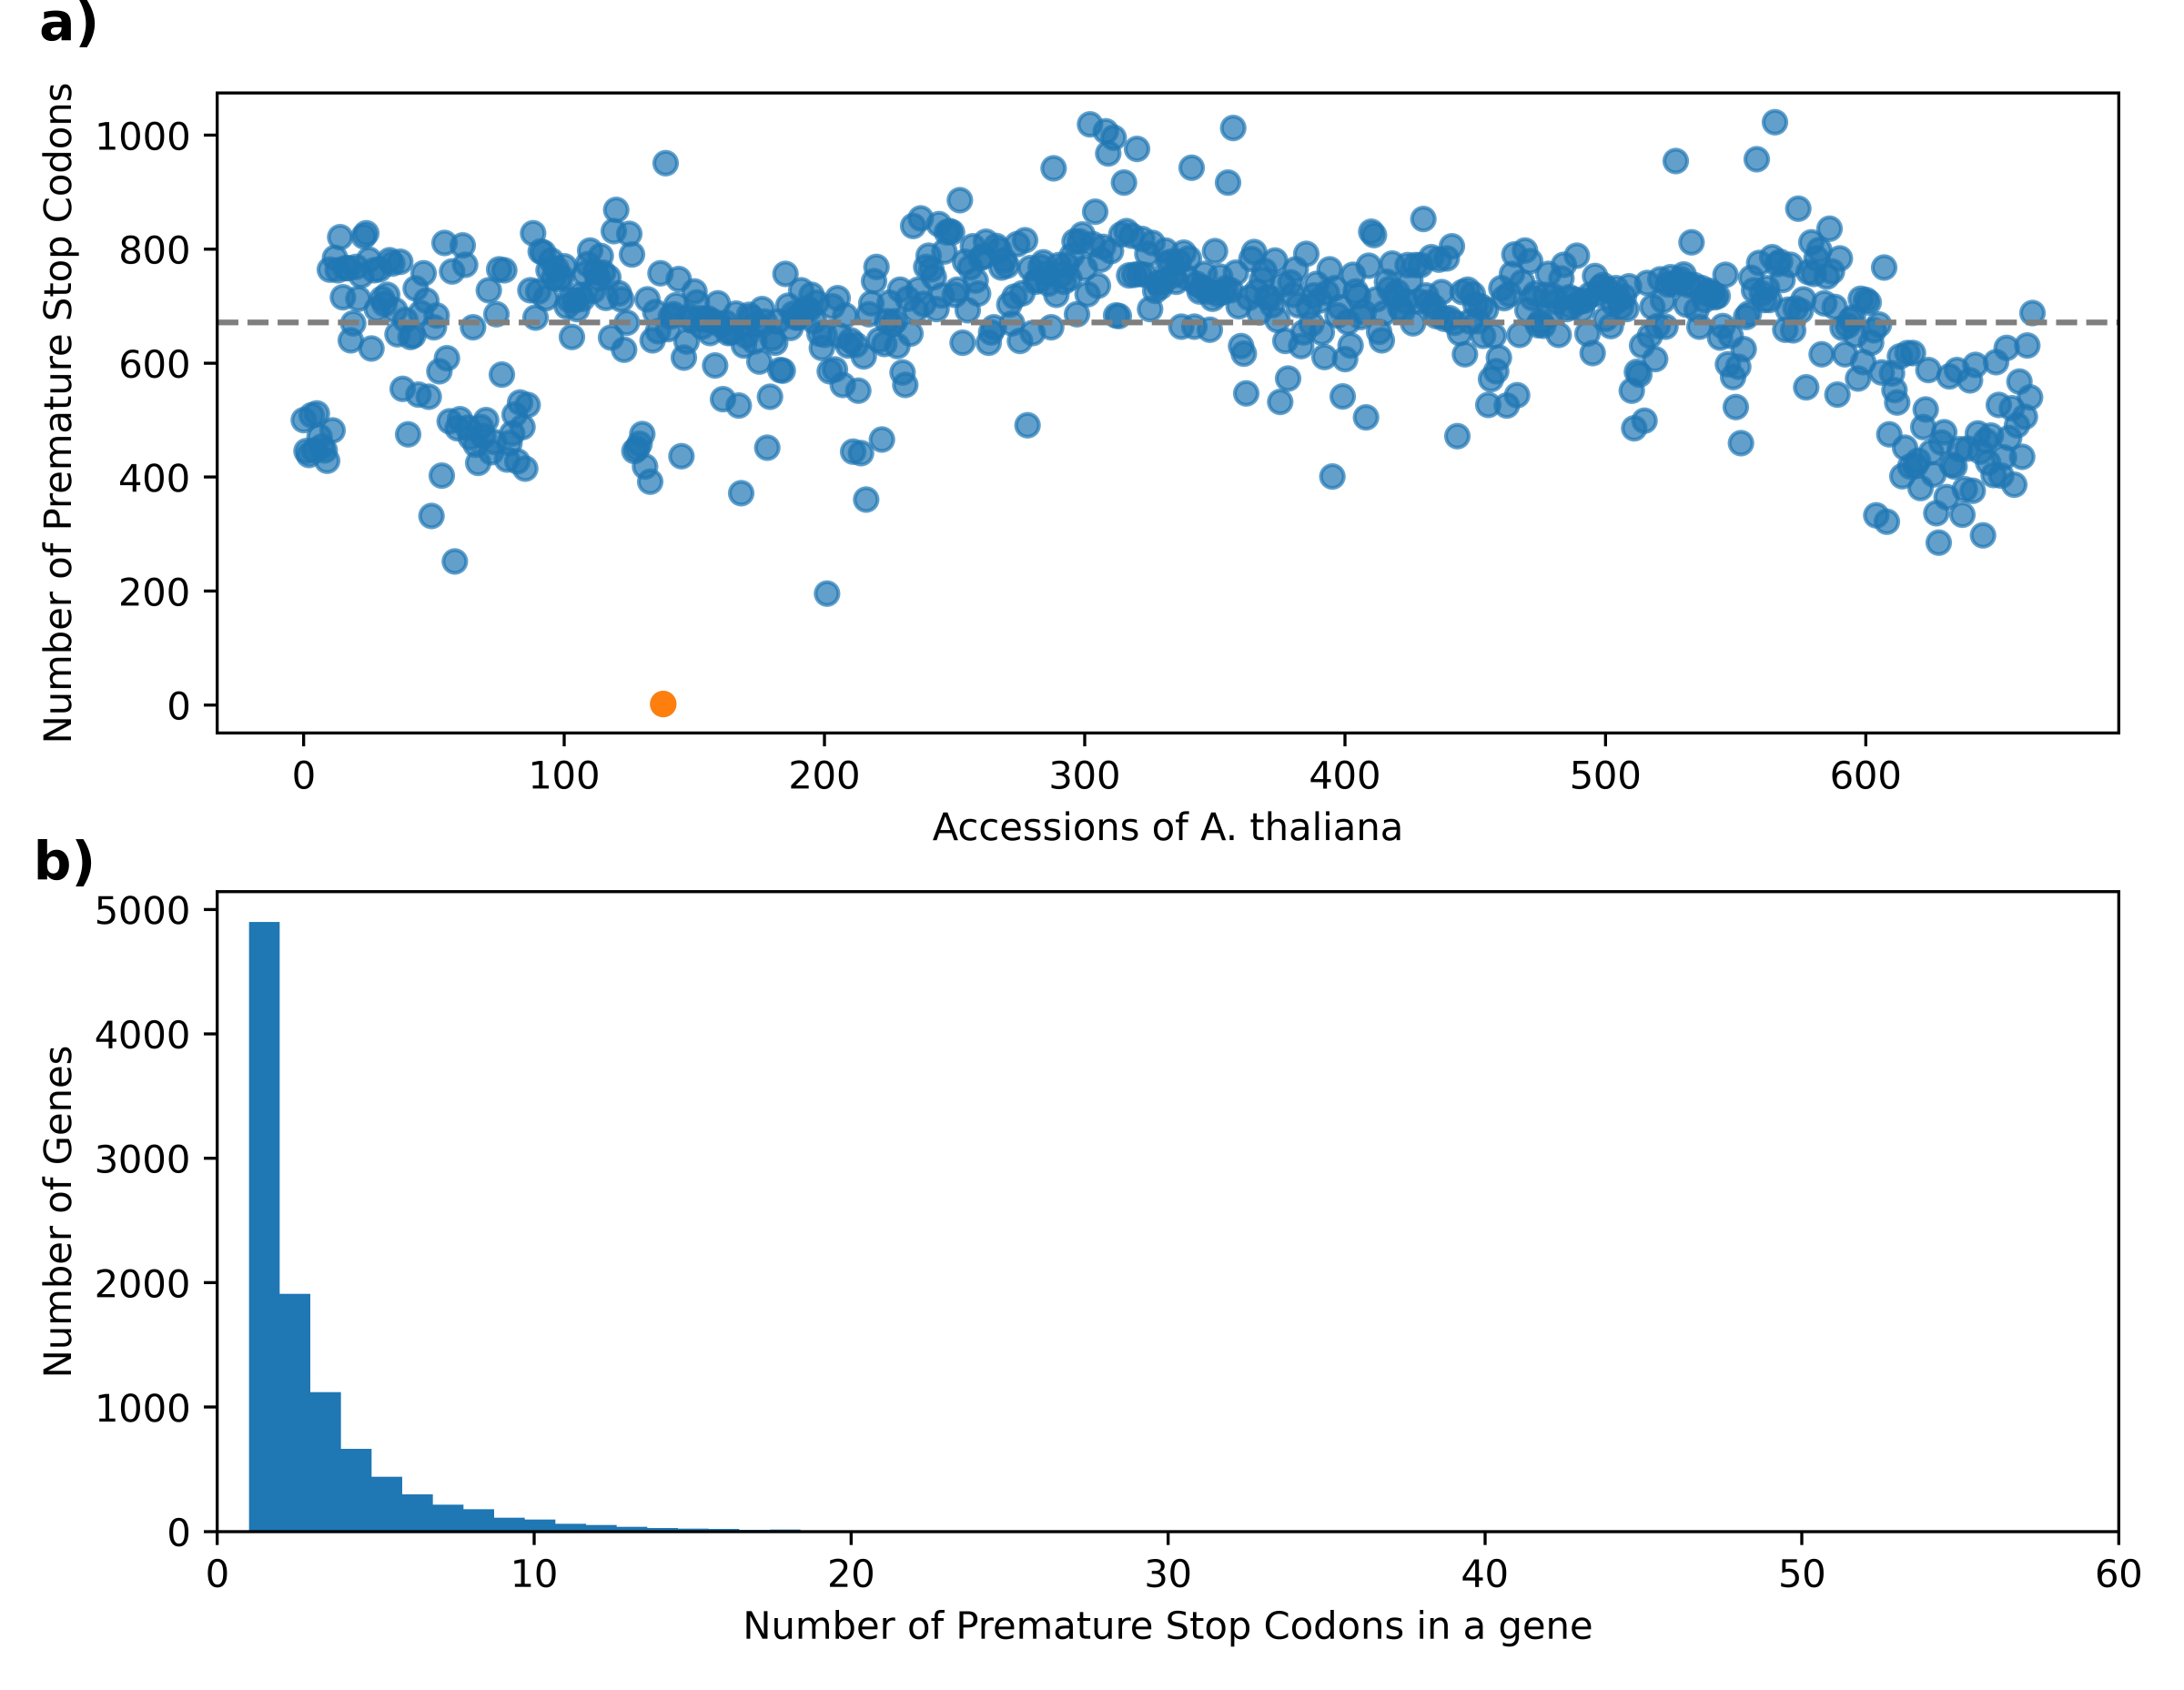
\includegraphics[width=1\textwidth]{images/Distribution_Premature_Stop_Codons.png}
      \caption[Distribution of premature stop codons in the genome from the 665 accessions \textit{A. thaliana} population]{\textbf{Distribution of premature stop codons in the genome from the 665 accessions \textit{A. thaliana} population}\\
      a) Distribution of premature stop codons along the 665 accessions. In each accessions, execept one, exist many hundreds of premature stop codons across the whole coding sequences of the genome. b) Histogram of number of stop codons in a gene. Most of the premature stop codons occur just once in each gene but there are also genes where we have multiple premature stop codons occurring. }
     \label{fig:Distribution_Premature_Stop_Codons_all}
    \end{minipage}
  \end{figure} 